\begin{frame}[fragile]
\frametitle{The Expression Problem}
\begin{block}{Cheat Detection}
lichess.org is an open-source chess server, written using Scala.
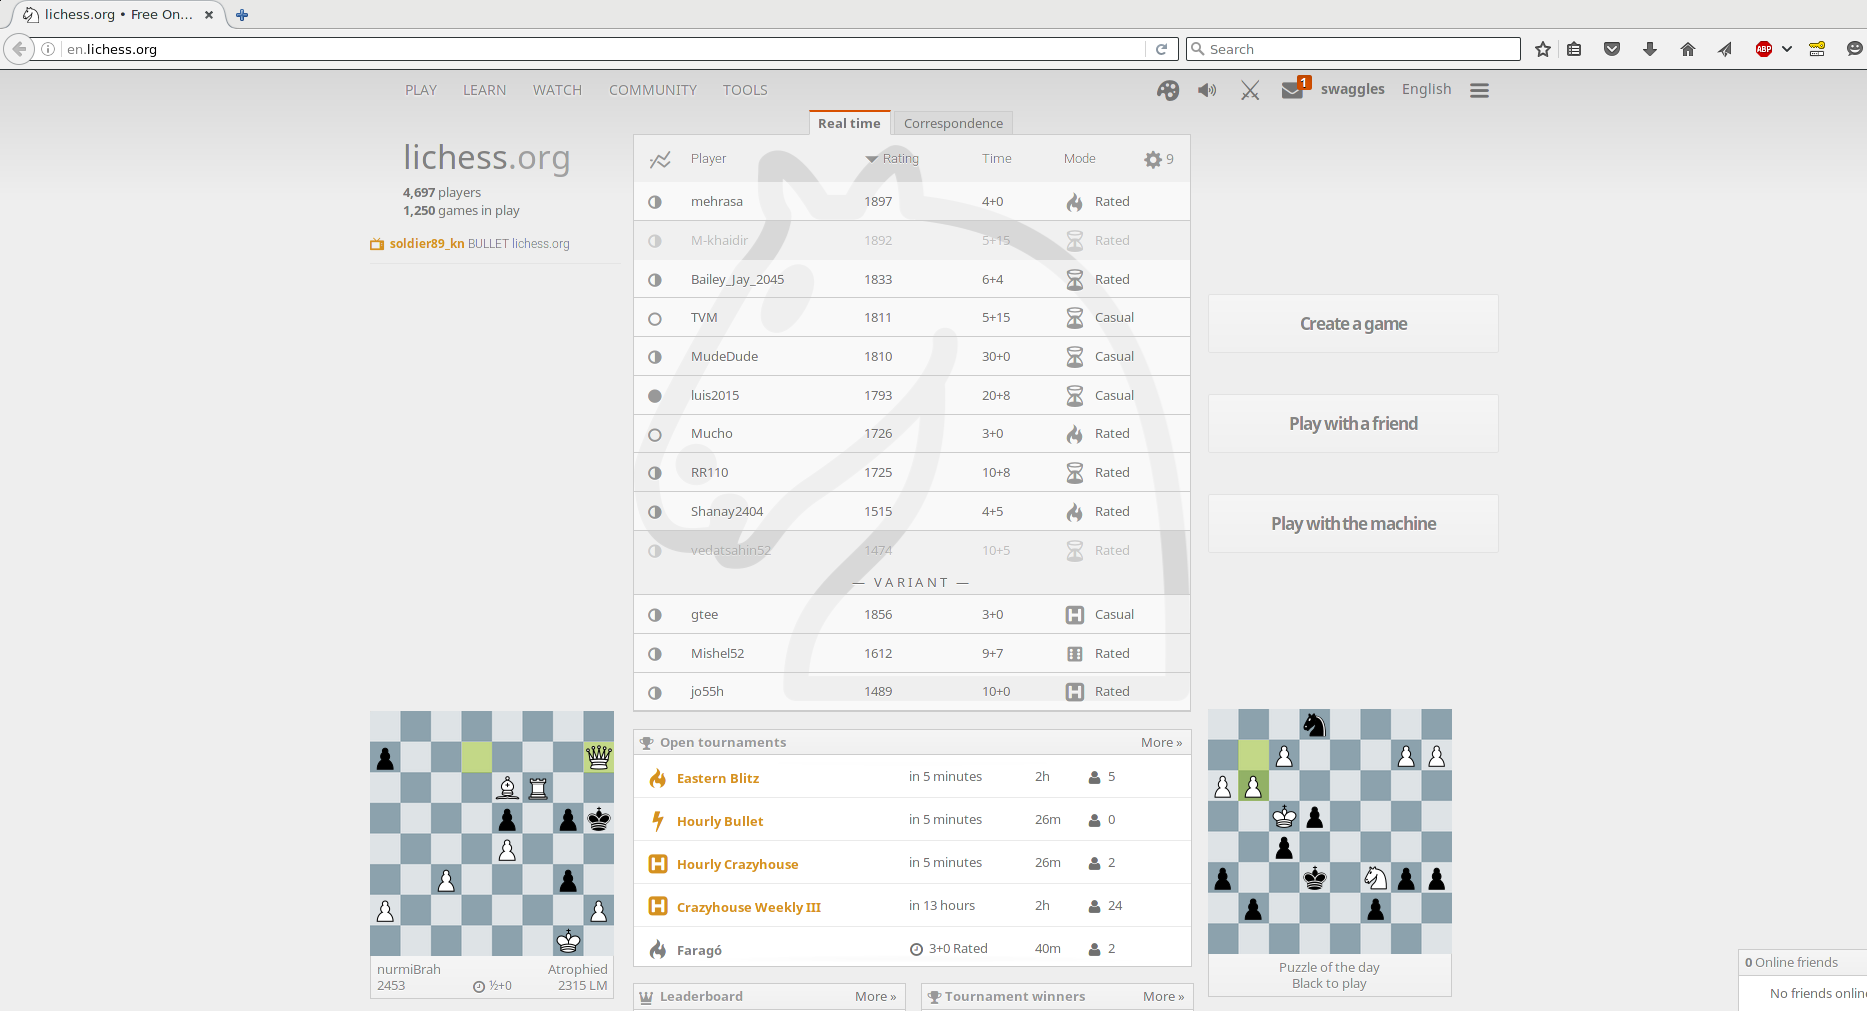
\includegraphics[height=0.4\textheight,natwidth=1867,natheight=1011]{image/lichess.png}
\end{block}
\end{frame}

\begin{frame}[fragile]
\frametitle{The Expression Problem}
\begin{block}{Cheat Detection}
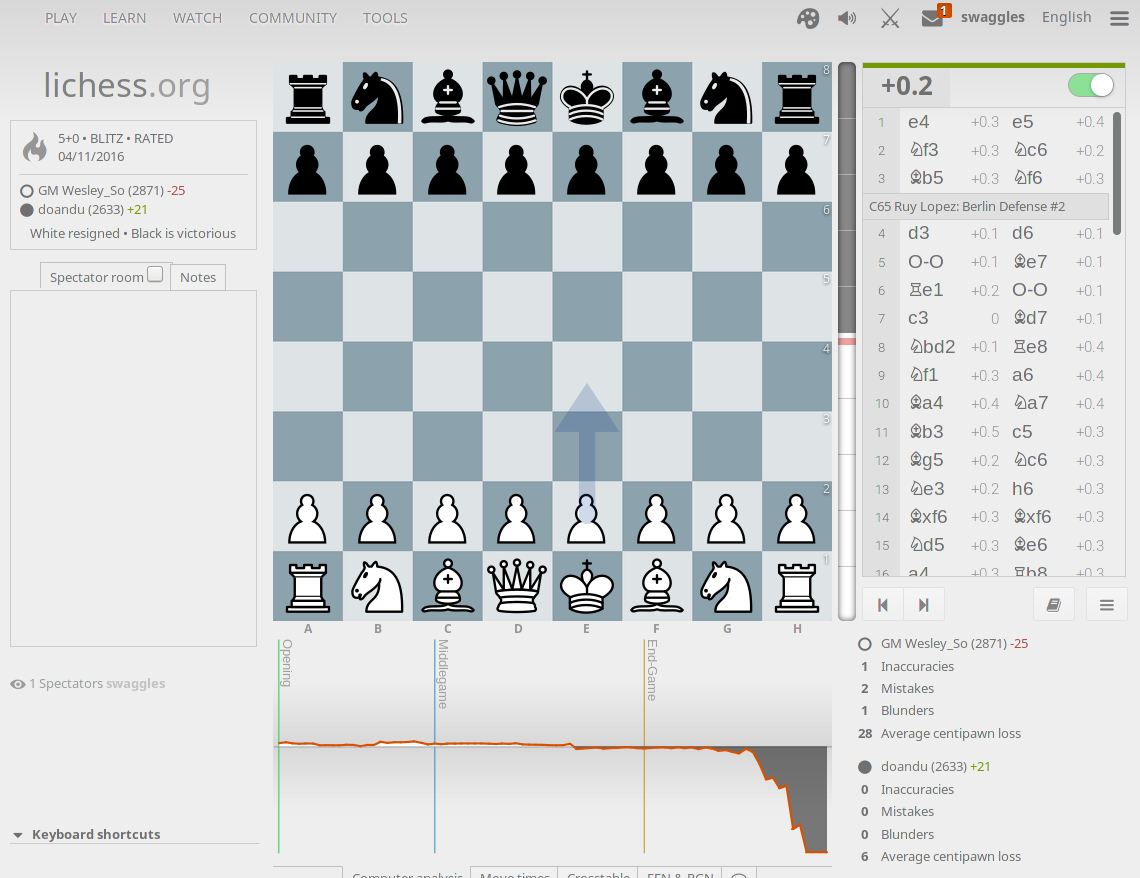
\includegraphics[height=0.5\textheight,natwidth=1140,natheight=878]{image/lichess-wesley-so.png}
\par
Here is the world \#12 being beaten by a patzer using computer-assistance.
\end{block}
\end{frame}

\begin{frame}[fragile]
\frametitle{The Expression Problem}
\begin{block}{Cheat Detection}

\includegraphics[height=0.2\textheight,natwidth=883,natheight=184]{image/lichess-wesley-so-announce.png}
\par
\end{block}
\end{frame}

\begin{frame}[fragile]
\frametitle{The Expression Problem}
\begin{block}{Cheat Detection}
\begin{lstlisting}[style=haskell,mathescape]
cheatReport :: String
\end{lstlisting}
Currently, cheat reports are written by and assessed by humans.
\end{block}
\end{frame}

\begin{frame}[fragile]
\frametitle{The Expression Problem}
\begin{block}{Cheat Detection}
\begin{lstlisting}[style=haskell,mathescape]
data CheatReport =
  UnhumanCriticalLine MoveNumber
  | RepeatingMoveStrengthPattern Pattern
  | UnusualCentipawnLoss Loss
  | $\ldots$
\end{lstlisting}
\end{block}
\end{frame}

\begin{frame}[fragile]
\frametitle{The Expression Problem}
\begin{block}{Cheat Detection}
\begin{itemize}
\item A \lstinline{String} cheat report provides open description.
\item However, with no structure, applying any automation is impossible.
\item A closed, structured cheat report afford automation.
\item However, cheat report structure is likely to change over time.
\end{itemize}
\end{block}
\end{frame}

\begin{frame}[fragile]
\frametitle{The Expression Problem}
\begin{block}{Cheat Detection}
\begin{lstlisting}[style=haskell,mathescape]
class AsMoveNumber p f s where $\ldots$
class AsCentipawnLoss p f s where $\ldots$
learn :: AsPattern p f s => $\ldots$
\end{lstlisting}
\end{block}
\end{frame}
